\documentclass[11pt,a4paper]{scrartcl}
\usepackage[czech]{babel}
\usepackage[utf8]{inputenc}
\usepackage{graphicx}
\usepackage{epstopdf}
\usepackage{float}
\graphicspath{{./img/}}

\begin{document}
	\title{Semestrální práce z předmětu KIV/NET}
	\subtitle{Dungeon hra}
	\author{Zdeněk Valeš - A17N0094P}
	\date{7. 4. 2018}
	\maketitle
	\newpage
	
	Souhlasím s vystavením této semestrální práce na stránkách katedry informatiky a výpočetní techniky a jejímu využití pro prezentaci pracoviště.
	
	\newpage
	
	\section{Zadání}
	V jazyce C\# vytvořte jednoduchou hru, ve které bude hráč procházet bludištěm (dungeonem). Cílem hráče je najít východ dříve než protihráči (počítač). Uživatelské rozhraní bude realizováno technologií WPF. Aplikace bude obsahovat jednoduchý editor map s možností importovat (exportovat) mapy do (ze) souboru.
	
	\subsection{Cíl projektu}
	Cílem projektu je vytvoření jednoduché hry. Při tvorbě aplikace se seznámím se základními technologiemi a postupy, které se v této oblasti používají.
	
	\subsection{Požadavky}
	Aplikace má následující funkční požadavky:
	\begin{itemize}
		\item Vytvořit novou hru o zadané velikosti mapy (šířka, výška), se zadaným počtem soupeřů (ovládaných počítačem).
		
		\item Hráč může při procházení mapou sbírat předměty, které mu pomáhají ve hře (zbroj, zbraně, klíče, ...).
		
		\item Vyhrát hru nalezením cílového pole, případně hru prohrát, pokud toto pole nalezne soupeř.
		
		\item Vytvořit mapu v editoru a vyexportovat ji do souboru.
		
		\item Importovat mapu ze souboru.
	\end{itemize}
	
	\section{Analýza}
	
	Jádro aplikace se skládá ze 3 hlavních komponent. 1. komponenta obsahuje vše potřebné pro práci s herní mapou, 2. obsahuje herní objekty (včetně hráčů), 3. pak instanci hry a herní mechaniky.
	
	\subsection{Komponenta pro práci s herní mapou}
	Herní mapa je tvořena maticí herních polí. Každé herní pole má čtyři východy (podle světových stran), které mohou být v otevřeném, zavřeném, nebo neexistujícím stavu a v jednom okamžiku se na něm může nacházet pouze jeden živý a jeden neživý objekt Hráč vidí pouze na přilehlé bloky, do kterých se může dostat. Jednotlivé stavy jsou popsány v následujícím výčtu:
	
	\begin{itemize}
		\item \textit{OTEVŘENÝ}: východ je otevřený a blok je možné tímto východem opustit, nebo do něj přijít.
		
		\item \textit{ZAVŘENÝ}: východ je zavřený a k jeho otevření je potřeba získat klíč (a mít jej v inventáři). Pokud je východ jednou otevřen pomocí klíče, nemůže být už znovu zavřen a každý jím může projít.
		
		\item \textit{NEEXISTUJÍCÍ}: východ v tomto směru neexistuje. V uživatelském rozhraní bude reprezentován například zdí.
	\end{itemize}

	
	\paragraph{Generování mapy}
	V aplikaci je dungeon vnímán jako podzemní bludiště (například systém jeskyní) a k vytvoření herní mapy je k dispozici generátor. 
	
	Ke generování mapy je použit algoritmus postupného probourávání, kdy na začátku je matice herních polí se všemi východy ve stavu \textit{NEEXISTUJÍCÍ} a algoritmus postupně prochází celou mapu a náhodně probourává stěny jednotlivých bloků. Výsledkem je bludiště bez izolovaných míst -- platí tedy, že mezi každými dvěma bloky existuje cesta. To mimo jiné zjednodušuje pozdější náhodou volbu startovacích pozic hráčů, monster a umístění předmětů, protože nemůže nastat situace kdy by například hráč nemohl dojít do cíle.
	
	\subsection{Komponenta pro práci s herními objekty}
	Všechny objekty, které mohou být umístěny na mapu, a v případě hráčů a monster se po ní mohou i pohybovat, jsou v rámci aplikace souhrnně nazvané jako 'herní objekty'. Jsou rozděleny do dvou podmnožin: živé a neživé objekty, kde živé objekty představují hráče (člověka i počítač), neživé pak předměty které lze na mapě sebrat (například zbraň).
	
	Všechny předměty mají dvě společné vlastnosti: hrací blok, na kterém jsou umístěné a název. Základní struktura herních objektů je naznačena na obrázku \ref{fig:game-obj}. 
	
	\begin{figure}[H]
		\centering
		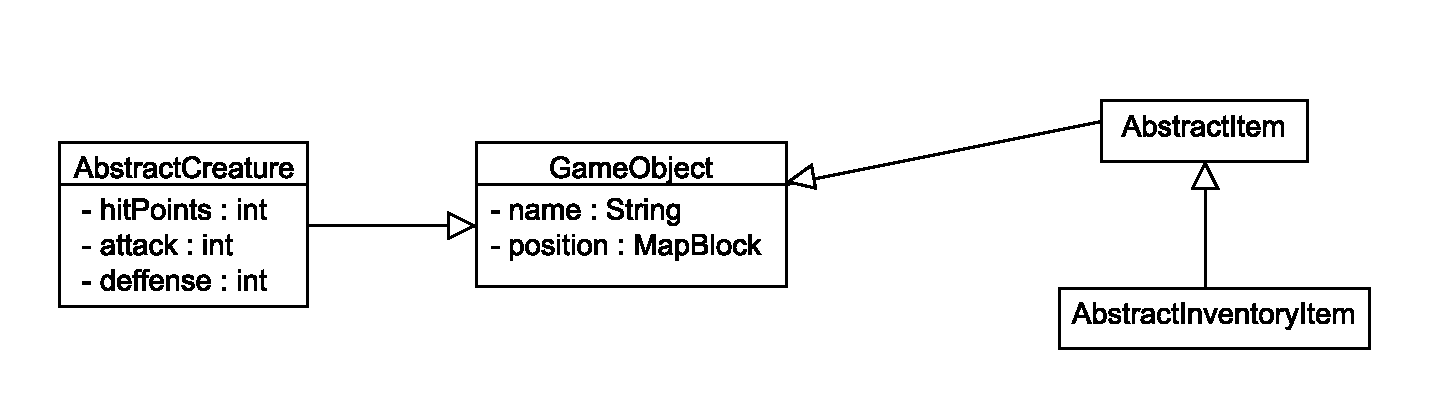
\includegraphics[width=140mm]{core-game-objects-simple}
		\caption{Struktura herních objektů}
		\label{fig:game-obj}
	\end{figure}
	
	\subsubsection{Předměty}
	Předměty může mít hráč buďto nasazené (na obrázku \ref{fig:game-obj} \textit{AbstractItem}), nebo je může nosit v inventáři (na obrázku \ref{fig:game-obj} \textit{AbstractInventoryItem}). 
	
	V případě nositelných předmětů se jedná o zbraně a brnění. Ty dávají hráči bonusy k jeho základním schopnostem (zdraví, útok, obrana). Hráč může mít v jeden okamžik nasazenou pouze jednu zbroj a jednu zbraň. Pokud má hráč nasazenou zbroj (zbraň), zvyšuje se jeho celková obrana (útok).
	
	Oproti tomu v inventáři může hráč nosit libovolný počet stejných věcí (počet je omezen kapacitou inventáře). Speciální věc v inventáři je pak klíč, který slouží k odemčení zavřených průchodů mezi herními bloky.
	
	\subsubsection{Monstra a hráči}
	Ve hře se vyskytují dva typy živých objektů - monstra a hráči. Monstra jsou 'jednodušší' verzí hráčů: nemají inventář, sloty na zbraně a brnění a ani nemohou vyhrát hru. Mohou se pohybovat po mapě a případně napadat ostatní hráče. Monstrum je také vždy ovládáno pouze počítačem, hráč může oproti tomu být ovládaný jak počítačem, tak člověkem.
	
	Chování monster je jednoduché: náhodně volí cestu a po dosažení určitého počtu bloků se vrátí na původní pozici. Tímto způsobem náhodně procházejí oblast (jejíž velikost je daná délkou cesty) kolem své startovní pozice. Oproti tomu hráč-počítač prochází bludiště algoritmem DFS. V současné verzi nesbírá žádné předměty a snaží se vyhýbat bitvám.
	
	\subsection{Komponenta s herní mechanikou}
	Herní mechanika je tvořena herní smyčkou a akcemi, které mohou hráči a monstra provádět. Poslední komponenta spojuje předchozí dvě a dohromady s nimi tvoří jádro celé hry.
	
			\begin{figure}[H]
				\centering
				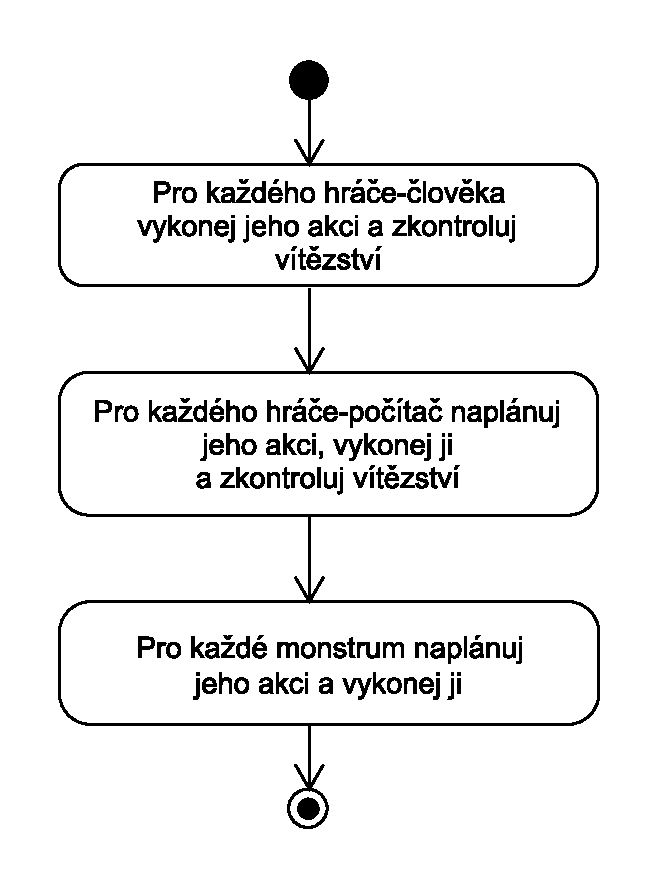
\includegraphics[height=75mm]{game-loop-simple}
				\caption{Jeden krok herní smyčky}
				\label{fig:game-loop}
			\end{figure}
	
	\subsection{Herní smyčka}
	Herní smyčka tvoří 'srdce' celé hry. Aby bylo možné jádro v budoucnu pohodlně propojit s uživatelským rozhraním, je implementován pouze jeden krok herní smyčky, který bude z UI cyklicky volán. 
	
	Krok herní smyčky je znázorněn na obrázku \ref{fig:game-loop}. V případě, že jeden z hráčů splní podmínku vítězství, krok skončí předčasně a je na vyšší vrstvě (uživatelském rozhraní), aby upozornila uživatele na konec hry.
	
	Plánování akcí a jejich vykonání lze teoreticky rozdělit do dvou oddělených smyček (tedy nejdříve se pro všechny hráče/monstra naplánují akce a pak se vykonají), ale pak se hra může dostat do situace, kdy si dvě monstra naplánují krok na stejné pole, nebo si hráč naplánuje útok na pole, kde již nikdo není. Aby se těmto situacím zamezilo, zvolil jsem způsob, kdy je akce vykonána hned po naplánování.
	
	
	\subsection{Herní akce}
	Jeden z nejjednodušších způsobů realizace herních akcí (pohyb, boj, sebrání předmětu) je implementovat tyto akce v příslušných entitách (\textit{AbstractCreature}, \textit{AbstractPlayer}). To by ovšem znamenalo přenesení většiny herní logiky do těchto tříd a později by to mohlo vést k znepřehlednění kódu a obtížné škálovatelnosti aplikace. Proto jsem se rozhodl využít návrhový vzor Command.
	
	Realizace každé herní akce je tak přesunutá do zvláštní entity a je závislá jen na objektech, kterých se týká. Každý hráč má pak vlastní frontu akcí, ze které hra postupně odebírá a jednotlivé akce provádí. Schéma herních akcí je zobrazeno na obrázku \ref{fig:game-act}.
	
	\begin{figure}[H]
		\centering
		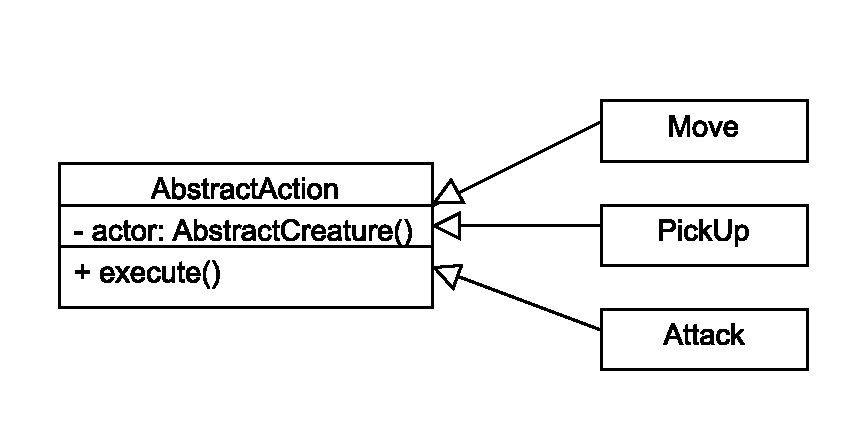
\includegraphics[height=35mm]{core-game-actions-simple}
		\caption{Schéma herních akcí}
		\label{fig:game-act}
	\end{figure} 
	
	\paragraph{Utočení} Útočit může hráč pouze na sousední bloky. K tomu stačí znát současnou pozici hráče a směr, kterým chce útočit. Výsledná hodnota útoku se spočítá podle vzorečku $poskozeni=max(0,utok_{utocnik} - obrana_{protivnik})$. Pokud protivník umřel, prohrává a hry se dále neúčastní.
	
	\section{Implementace}
	
	Aplikace se skládá ze dvou hlavních částí - jádro a uživatelské rozhraní. Jádro je řešené jako samostatná knihovna (Class library), kterou lze 'připojit' k uživatelskému rozhraní. V současné době je implementováno pouze jádro aplikace.
	
	\subsection{Komponenta pro práci s herní mapou}
	Komponenta pro práci s herní mapou se skládá z datových tříd (\verb|Map|, \verb|MapBlock|, \verb|Entrance|, ...), které slouží ke generování mapy a z knihovní třídy \verb|MapSerializer|, která slouží k načítání a ukládání mapy do souboru.
	
	Každý herní blok má čtyři východy, k pohodlnému přístupu k těmto východům slouží výčet \verb|Direction|, který obsahuje čtyři světové strany. Tento výčet je navíc rozšířen o statickou třídu \verb|DirectionMethods|, která poskytuje metody pro usnadnění práce se směry. Schéma tříd týkajících se datového modelu herní mapy je naznačeno na obrázku \ref{fig:core-map}.
	
	\begin{figure}[H]
		\centering
		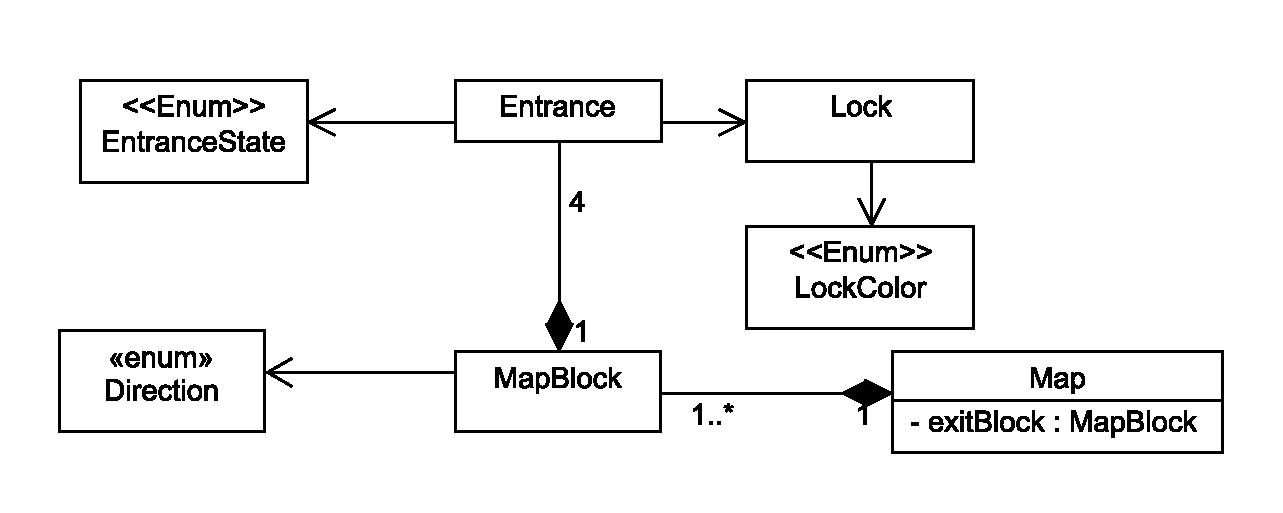
\includegraphics[height=40mm]{core-map-simple}
		\caption{UML diagram herní mapy}
		\label{fig:core-map}
	\end{figure}
	
	
	
	\subsubsection{Generování mapy}
	Metody pro generování map jsou deklarovány v rozhraní \verb|IMapGenerátor|. V současné verzi existují dvě implementace tohoto rozhraní. První, \verb|OpenMapGenerator|, vytvoří prázdnou mapu se všemi průchody otevřenými a slouží hlavně pro testování. Druhá, \verb|SimpleMapGenerator| pak generuje bludiště algoritmem popsaným v analytické části (zatím bez předmětů a protihráčů). UML diagram tříd týkajících se generování map je znázorněn na obrázku \ref{fig:core-map-generator}.
	
	\begin{figure}[H]
		\centering
		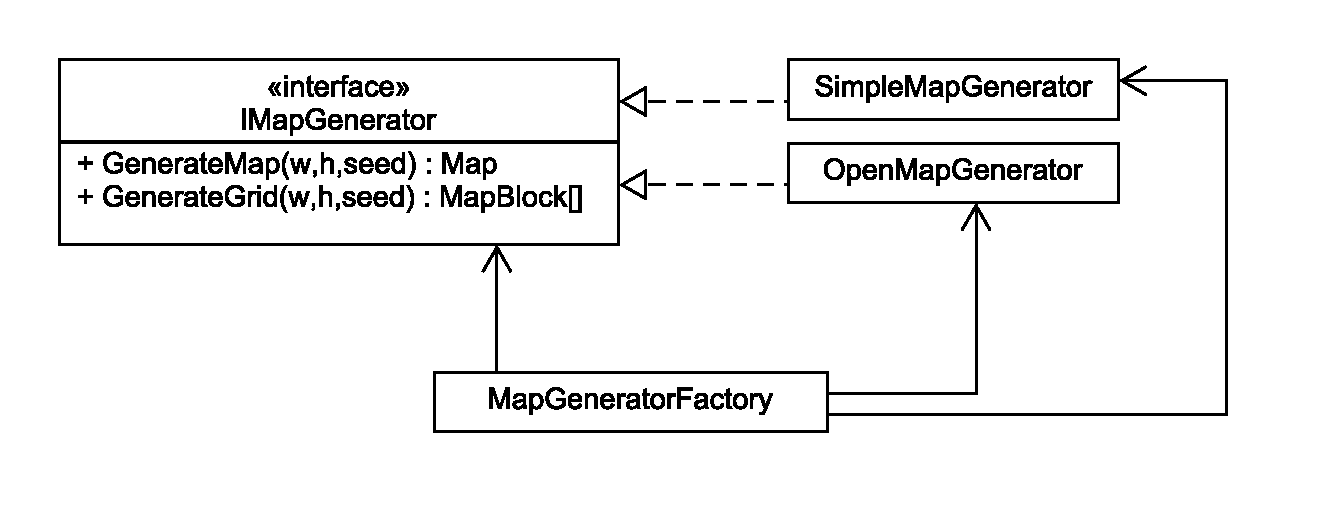
\includegraphics[height=40mm]{core-map-generator-simple}
		\caption{UML diagram generátorů herní mapy}
		\label{fig:core-map-generator}
	\end{figure}
	
	\subsubsection{Ukládání mapy}
	Ukládání mapy do souborů (a stejně tak její načítání) je řešeno serializací do formátu JSON pomocí knihovny Newtonsoft.Json. Původní záměr byl použít serializaci do XML pomocí standardních knihoven frameworku .NET, ale bohužel se mi nepodařilo do class library s jádrem přidat požadovanou závislost.
	
	V jádře je implementována pouze serializace do řetězce, uložení tohoto řetězce do souboru (nebo kamkoliv jinam) pak závisí na vrstvě, která bude jádro hry používat.
	
	\subsection{Komponenta pro práci s herními objekty}
	Jak již bylo zmíněno v analytické části, předměty ve hře se dělí na živé a neživé. Základem pro všechny objekty je třída \verb|GameObject|, která každému objektu dává jméno a pozici na mapě.
	
	\subsubsection{Monstra a protihráči}
	Nepřátelé jsou pro hráče-člověka monstra a ostatní hráči ovládaní počítačem. Monstrum je implementováno třídou \verb|Monster| a k vytvoření různých druhů monster slouží třída \verb|MonsterFactory|. jednotlivá monstra se od sebe liší pouze jménem a vlastnostmi (život, útok, obrana). Na obrázku \ref{fig:core-creatures} je pro úplnost zobrazen UML diagram znázorňující strukturu živých objektů.
	
	\begin{figure}[H]
		\centering
		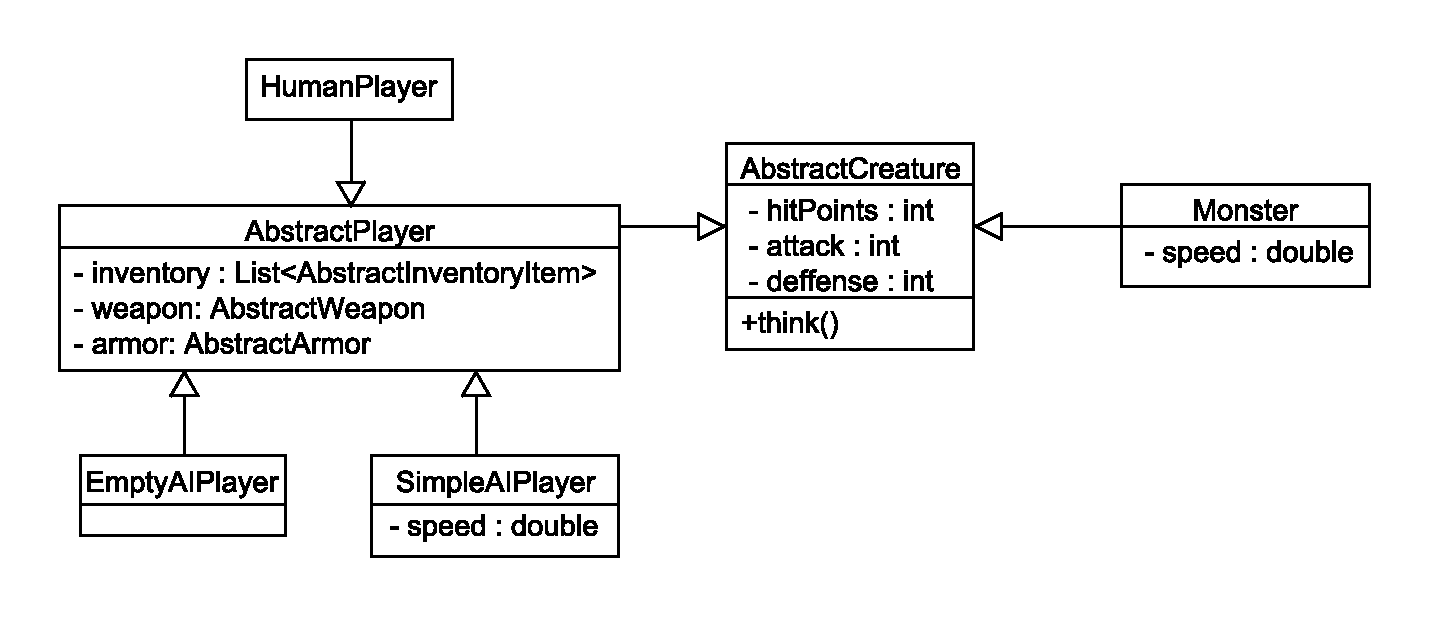
\includegraphics[width=140mm]{core-creatures-simple}
		\caption{UML diagram živých objektů}
		\label{fig:core-creatures}
	\end{figure}
	
	V současné době existují dvě implementace protihráčů: \verb|EmptyAIPlayer|, který nedělá nic a slouží k testování a \verb|SimpleAIPlayer|, který algoritmem DFS prochází mapu a snaží se najít východ. 
	
	\subsection{Komponenta s herní mechanikou}
	Instance herní třídy a krok herní smyčky je implementován ve třídě \verb|Game|. Jak již bylo zmíněno v analytické části, herní logika je implementována pomocí akcí. V případě výjimečných stavů produkují tyto akce výjimky, které by měla zachytit vrstva s uživatelským rozhraním a hráči chybu vhodně oznámit (například plný inventář, zavřený východ, ...).
	
	V případě, že některý z hráčů dojde do cílového pole (které nemusí být určeno - v takovém případě se jedná o nekonečnou hru), nastaví instance hry příznak \verb|IsWinner|. Opět je na vrstvě, která herní jádro využívá, aby po každém volání kroku herní smyčky zkontrolovala, zdali někdo nevyhrál.
	
	\subsection{Herní akce}
	Základní třída pro každou herní akci je \verb|AbstractAction|. Deklaruje metodu \verb|execute()|, kterou se akce vykoná a umožňuje nastavit objekt \verb|AbstractCreature|, nad kterým se akce vykoná (tedy ten, kdo akci provede). V současné době jsou implementovány akce na pohyb, útok a sebrání předmětu.
	 
	\section{Závěr}
	Jádro aplikace se povedlo naimplementovat a jeho základní funkcionalita je ověřena jednotkovými testy. V následující verzi přibude uživatelské rozhraní, které umožní hraní hry.
	
\end{document}
